\documentclass{article}
\usepackage[utf8]{inputenc}
\usepackage{graphicx} 
\usepackage{listings}
\usepackage{color}
\usepackage{float}
\usepackage{siunitx}
\graphicspath{{images/}}

\definecolor{dkgreen}{rgb}{0,0.6,0}
\definecolor{gray}{rgb}{0.5,0.5,0.5}
\definecolor{mauve}{rgb}{0.58,0,0.82}

\lstset{frame=tb,
  aboveskip=3mm,
  belowskip=3mm,
  showstringspaces=false,
  columns=flexible,
  basicstyle={\small\ttfamily},
  numbers=none,
  numberstyle=\tiny\color{gray},
  keywordstyle=\color{blue},
  commentstyle=\color{dkgreen},
  stringstyle=\color{mauve},
  breaklines=true,
  breakatwhitespace=true,
  tabsize=3
}

\title{RTR108 - Circuit Simulation Report}
\author{Bruno Bevilacqua Nascimento}
\date{March 2020}

\begin{document}

\maketitle

\section{Introduction}

In this report, it will be explained how to do circuit simulations using \textit{gschem} and \textit{ngspice} software.

\section{Body}

\subsection{Creating circuit using \textit{gschem}}

First, we need to open gschem software for creating a circuit. The circuit chosen in this report is a \textbf{High-Pass Filter} Circuit composed by the following components: \break

\begin{itemize}
\item  Voltage Source 10V (1kHz);
\item  Capacitor 3,3nF;
\item  Resistor \SI{1000}{\ohm}. 
\end{itemize} 

The \textit{Figure 1} shows the schematic drawing of the circuit.

\begin{figure}[H]
\centering
\includegraphics[width=1\textwidth, height=1\textwidth, angle =-90]{01}
\caption{High-Pass Filter Circuit}
\end{figure}

\subsection{Generating \textit{netlist}}

In order to generate your \textit{netlist}, execute the command below. \break

\begin{lstlisting}
## Command to generate gnetlist
getlist -g spice-sdb -o outputFile.net circuitSimulated.sch
\end{lstlisting} 

The final result for file \textit{.net} can be seen above: \break

\begin{lstlisting}
* gnetlist -g spice-sdb -o testCircuit.net testCircuit.sch
*********************************************************
* Spice file generated by gnetlist                      *
* spice-sdb version 4.28.2007 by SDB --                 *
* provides advanced spice netlisting capability.        *
* Documentation at http://www.brorson.com/gEDA/SPICE/   *
*********************************************************
*==============  Begin SPICE netlist of main design ============
v1 0 n0 SIN(0 10 1000Hz)
.INCLUDE ./Simulation.cmd
R1 0 n1 1k
C1 n0 n1 3.3nF
.end
\end{lstlisting} 

\subsection{Simulate circuit using \textit{ngspice}}

In order to simulate circuit, we are going to use \textit{ngspice}.
Execute \textit{ngspice} command in order to start the software and begin simulation. \break

\begin{lstlisting}
ngspice outputFile.net
\end{lstlisting} 

After this, you can execute \textit{run} command and see the result. \break

\begin{figure}[H]
\centering
\includegraphics[width=0.9\textwidth, height=0.9\textwidth, angle =0]{finalResults}
\caption{\textit{Ngspice} final results}
\end{figure}

With the defined nodes, we can plot the behaviour of our function typing the following command: \break

\begin{lstlisting}
plot n0 n1 v1#branch
\end{lstlisting} 

The software will generate the following graph.

\begin{figure}[H]
\centering
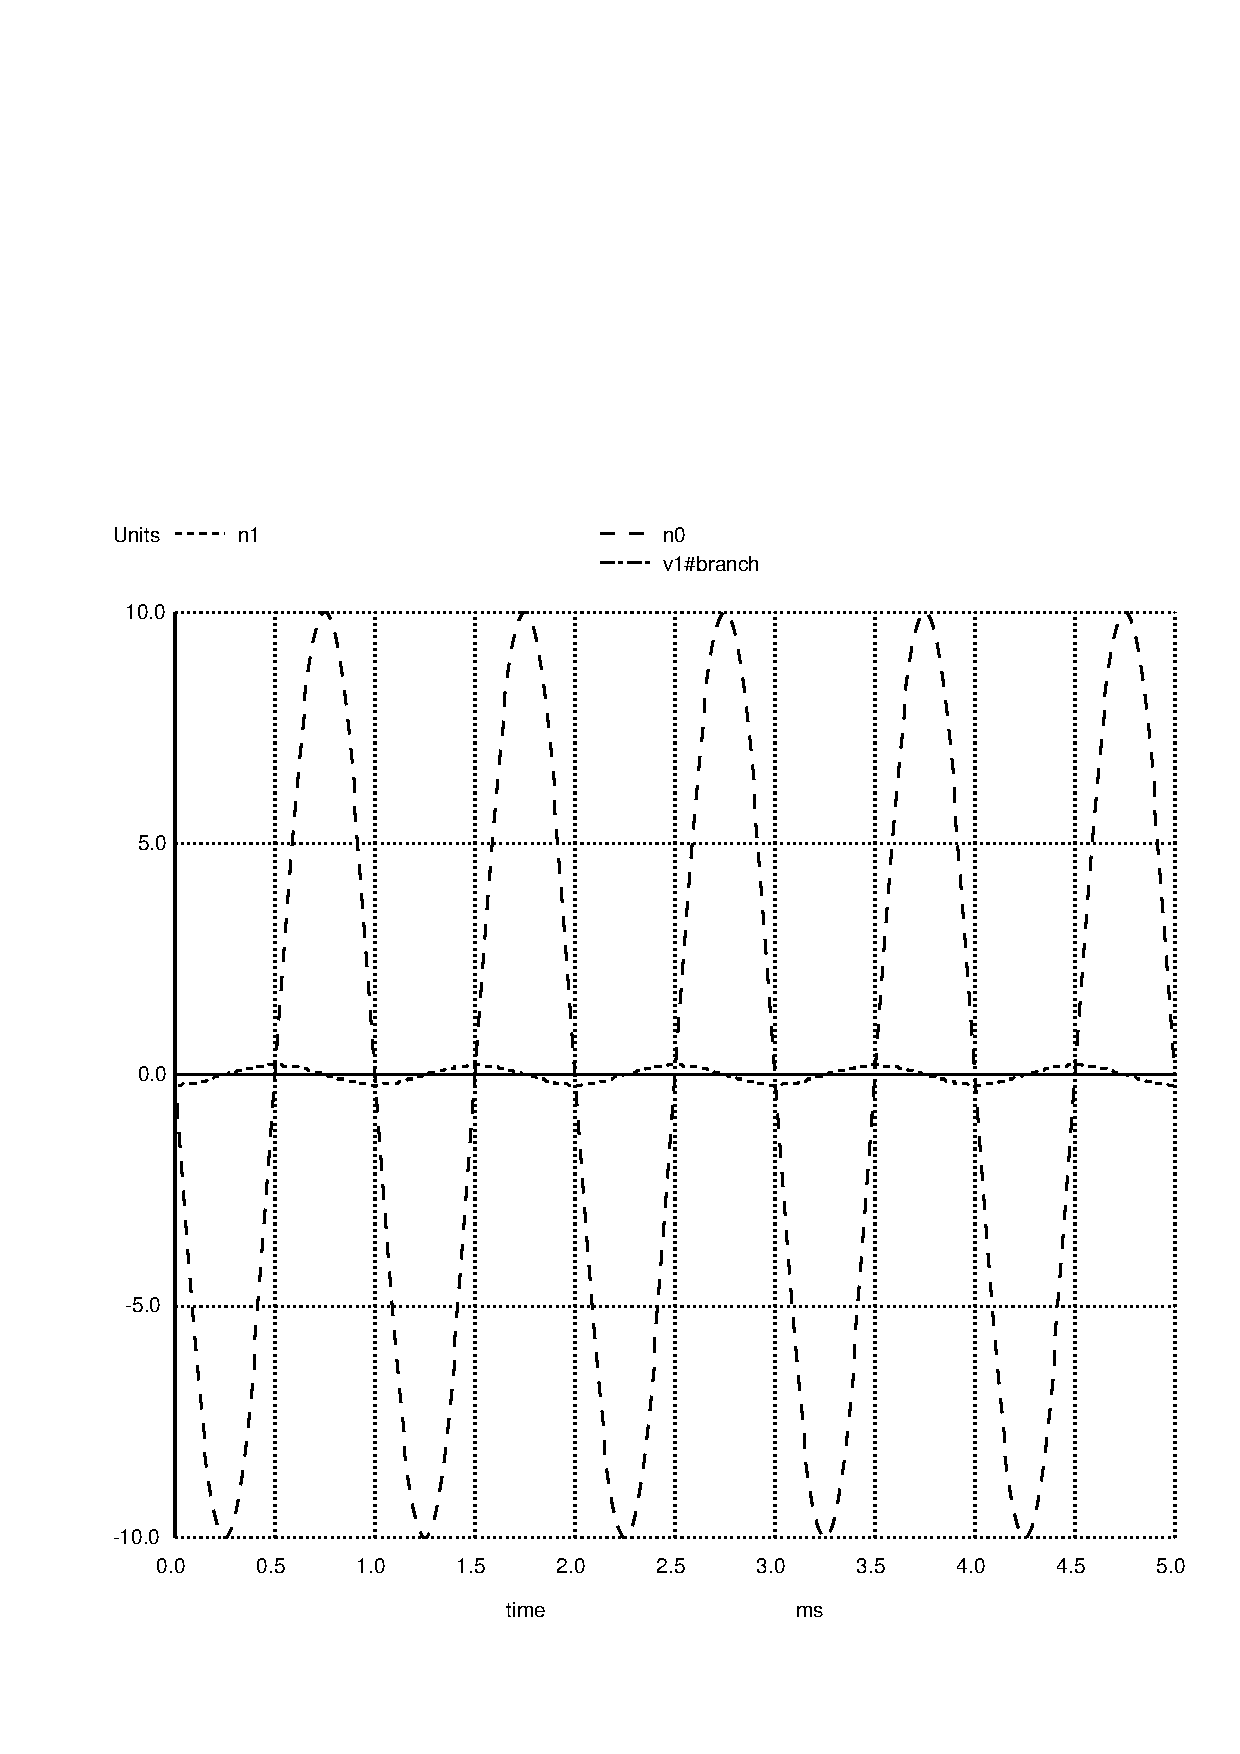
\includegraphics[width=0.5\textwidth, height=0.5\textwidth, angle =0]{011}
\caption{Complete graph of the circuit simulate}
\end{figure}

In order to see the entry signal you can execute the following command. \break

\begin{lstlisting}
plot n0
\end{lstlisting} 

\begin{figure}[H]
\centering
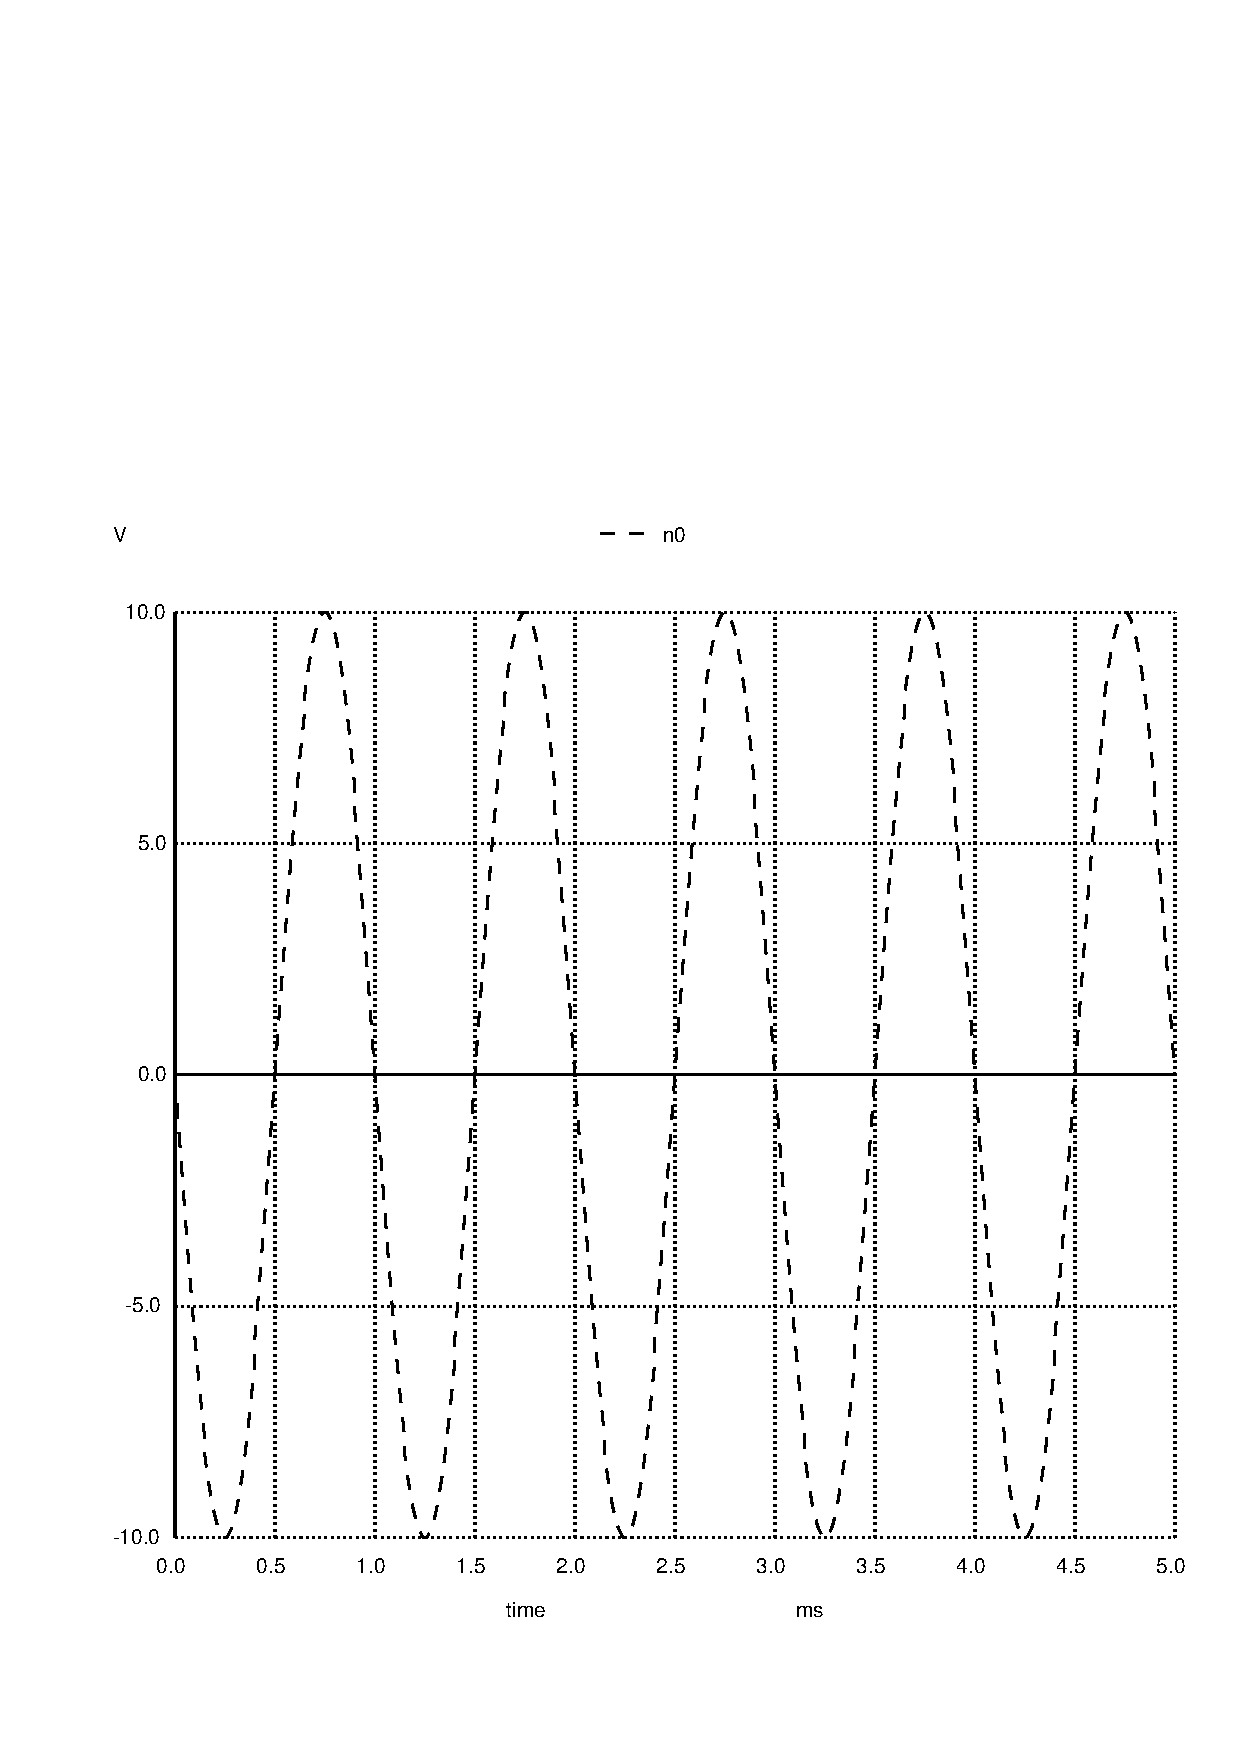
\includegraphics[width=0.5\textwidth, height=0.5\textwidth, angle =0]{012}
\caption{Entry signal \textit{n0}}
\end{figure}

In order to see the final signal you can execute the following command. \break

\begin{lstlisting}
plot n1
\end{lstlisting} 

\begin{figure}[H]
\centering
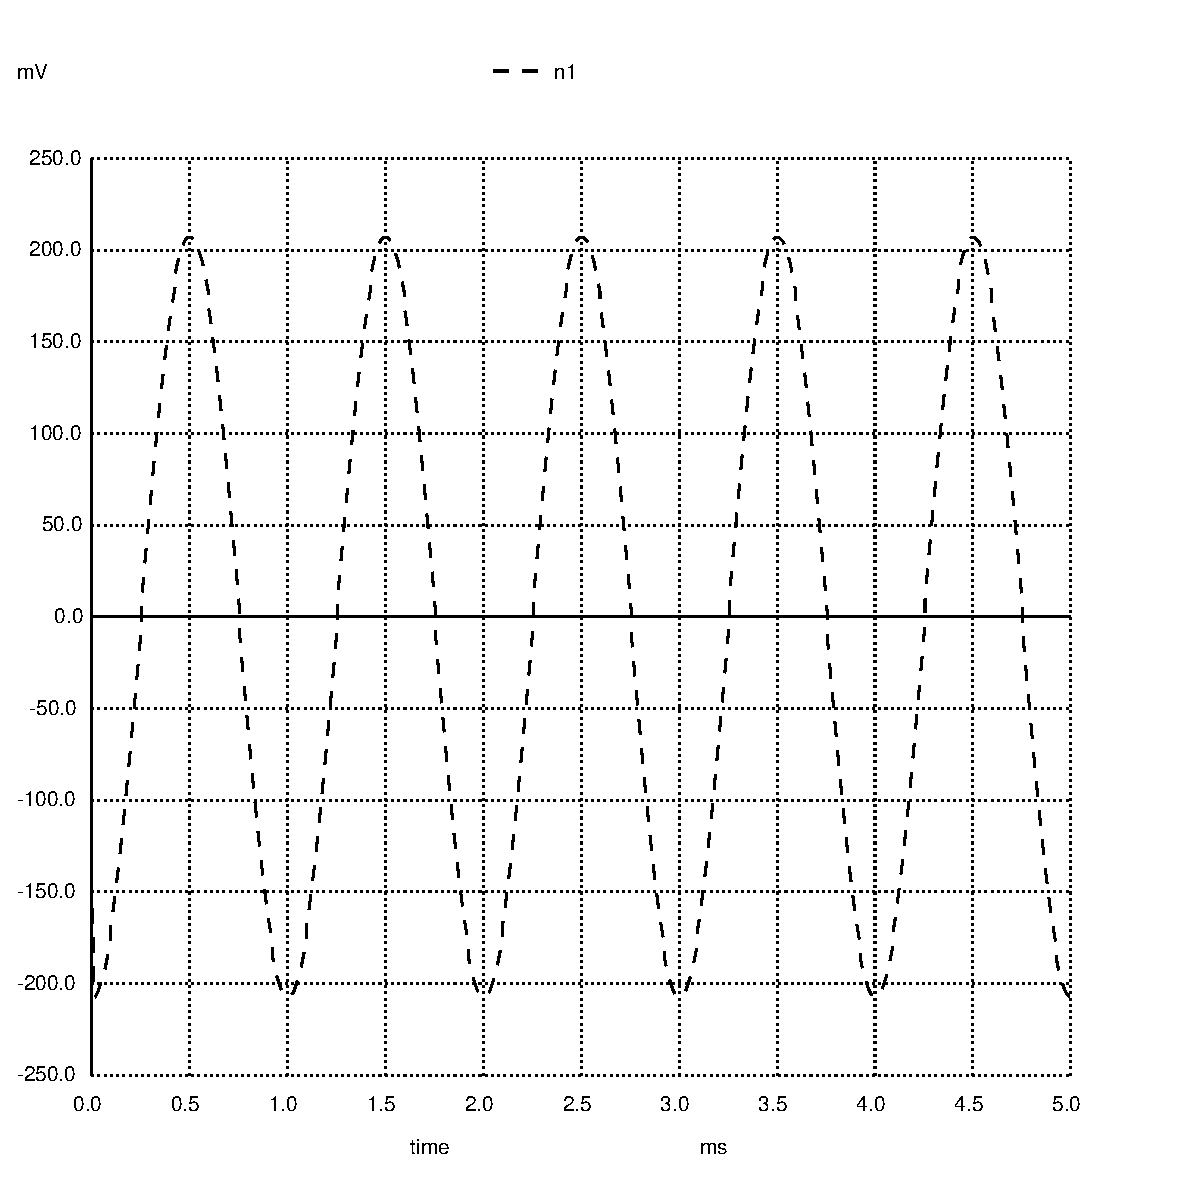
\includegraphics[width=0.5\textwidth, height=0.5\textwidth, angle =0]{013}
\caption{Final signal \textit{n1}}
\end{figure}

\section{Conclusion}

In this report it was shown how to simulate a circuit.
The chosen circuit was \textbf{High-Pass Filter} composed by a capacitor, resistor and a voltage source.
In the final result of circuit simulation we can see the difference between the two graphs (\textit{Figure 4} and \textit{Figure 5}). The entry signal has an amplitude of 10V, same of the voltage source. Otherwise, final signal has an amplitude of 200mV.
In order to see the same amplitude we need to increase frequency. For example, if we increase the frequency to 100kHz, entry signal and final signal will overlap like the graph below.

\begin{figure}[H]
\centering
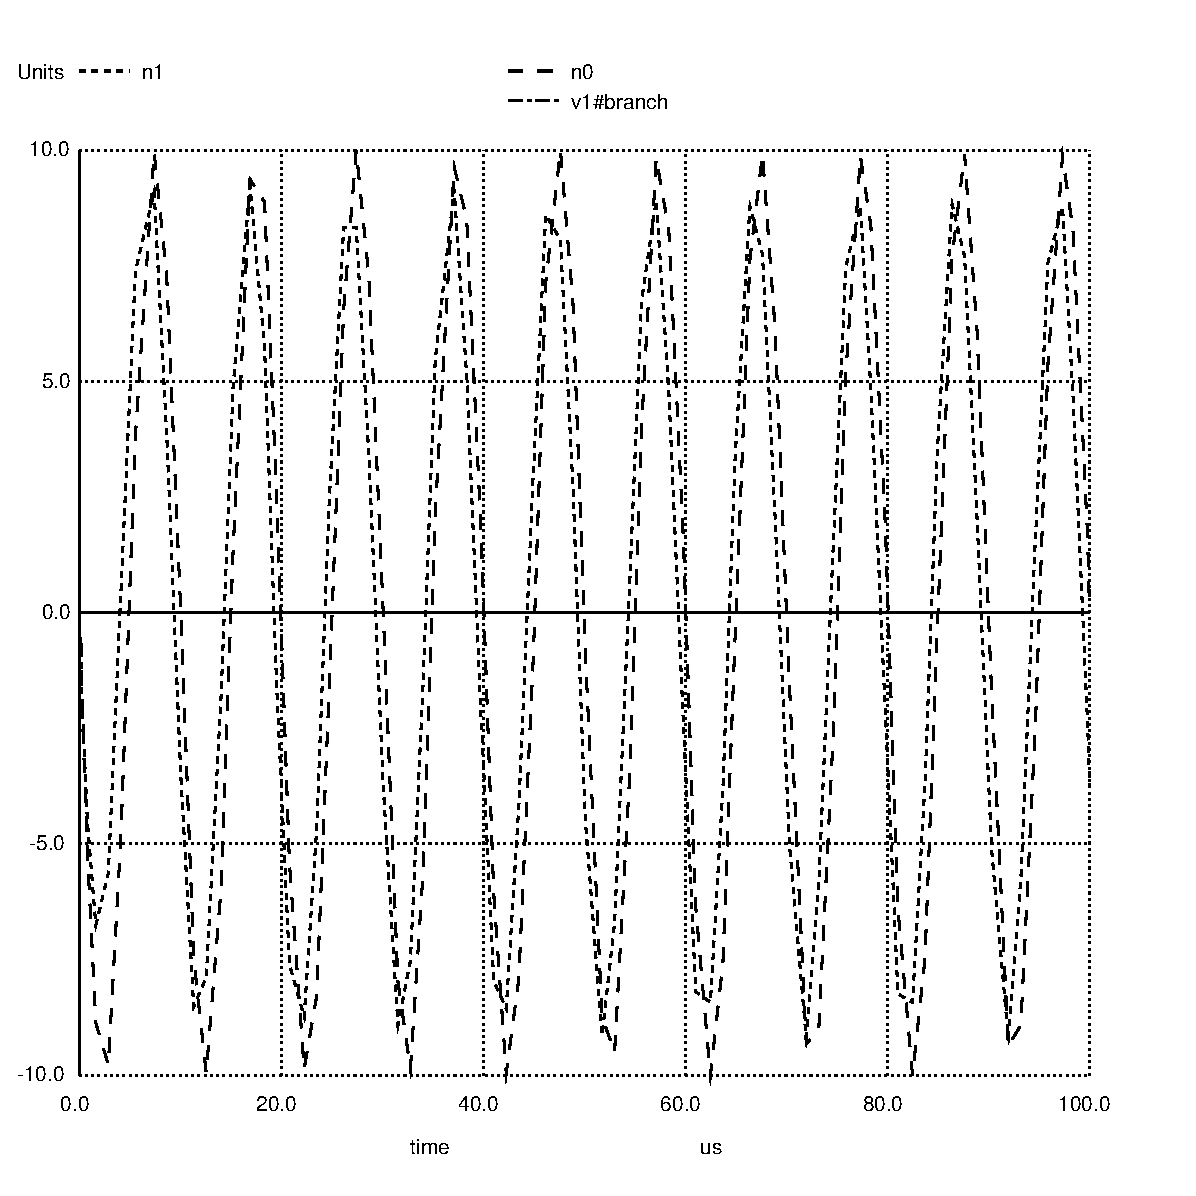
\includegraphics[width=0.5\textwidth, height=0.5\textwidth, angle =0]{014}
\caption{Entry signal and final signal overlapping for a frequency of 100kHz}
\end{figure}

Both of signals have amplitude of 10V. 
\break
So, in this report we could see a simulation of a \textbf{High-Pass Filter} and know how to simulate using \textit{gschem} and \textit{ngspice}. Basically, in order to generate your circuit you will have to follow the step-by-step below.
\break
\begin{enumerate}
\item Draw Circuit using \textit{gschem};
\item Generate netlist using \textit{gnetlist};
\item Simulate circuit using \textit{ngspice};
\item Analyze your results.
\end{enumerate}


\end{document}
